%%%%%%%%%%%%%%%%%%%%%%%%%%%%%%%%%%%%%%%%%%%%%%%%%%%%%%%%%%%%%%%%%%%
%                                                                 %
%                            CHAPTER FIVE                         %
%                                                                 %
%%%%%%%%%%%%%%%%%%%%%%%%%%%%%%%%%%%%%%%%%%%%%%%%%%%%%%%%%%%%%%%%%%%

\chapter{Data Volatility}

\section{Determining Volatility}

According to the Keyword Governance and Community Guide Document \ref{gcmd_gov}, “Full GCMD keywords list releases get a new major version number (e.g., 8.0). Incremental releases for updates to topics, terms, and variables get a new minor version number (e.g., 8.1).”  This explains the activity in Cluster 1 where there are sufficient changes to warrant a full release of the keywords.  Cluster 2 captures the change rate and duration of minor versions, except those from 8.2 to 8.4.1 which are in Cluster 3.  Cluster 3 demonstrates a flurry of activity occurring between June 7, 2016, to August 2, 2016.  Considering the previous pattern of taking at least six months between releases, three minor version releases within as many months is highly unusual.  An immediate concern is that Cluster 3 does not result from a sudden incident, resulting in increased activity.  An inquiry into reasoning behind the successive publication returned a statement that the government customer had requested this action.  Investigation into these versions required a look into their associated impact assessment reports.  Impact assessments prior to Version 8.5 are not publicly available, and only assessments for versions 8.2, 8.3, and 8.4 were received upon request.  Of the 6 requests affecting Earth Science Keywords in 8.2, published June 7, 2016, 4 were made in 2014, and the remaining 2 were made in 2015.  Version 8.3 had 8 entries in its impact assessment with 7 entries originating in 2014, and the remaining entry from 2015.  The 6 entries 8.4’s impact assessment has 5 entries from 2008 and 1 entry from 2015.

\begin{figure}%[b]
	\centering
	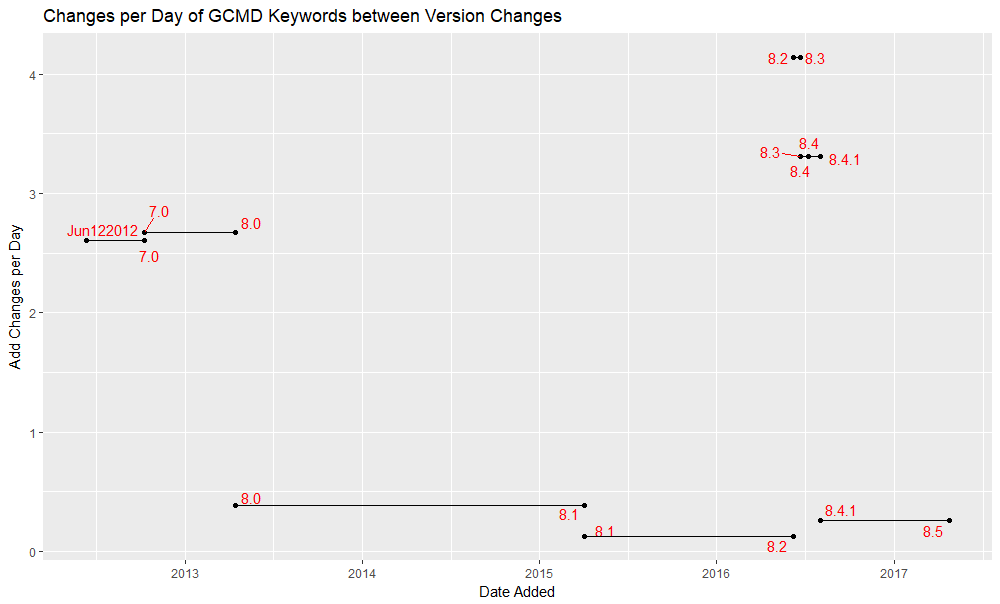
\includegraphics[scale=0.56]{figures/GCMDPlot1.png}
	\caption[Global Change Master Direcotry counts distributed over time.]{Add counts for all versions of GCMD up to 8.5 evenly distributed over the time of version validity.}
	\label{GCMDPlot1}
\end{figure}
\begin{figure}%[b]
	\centering
	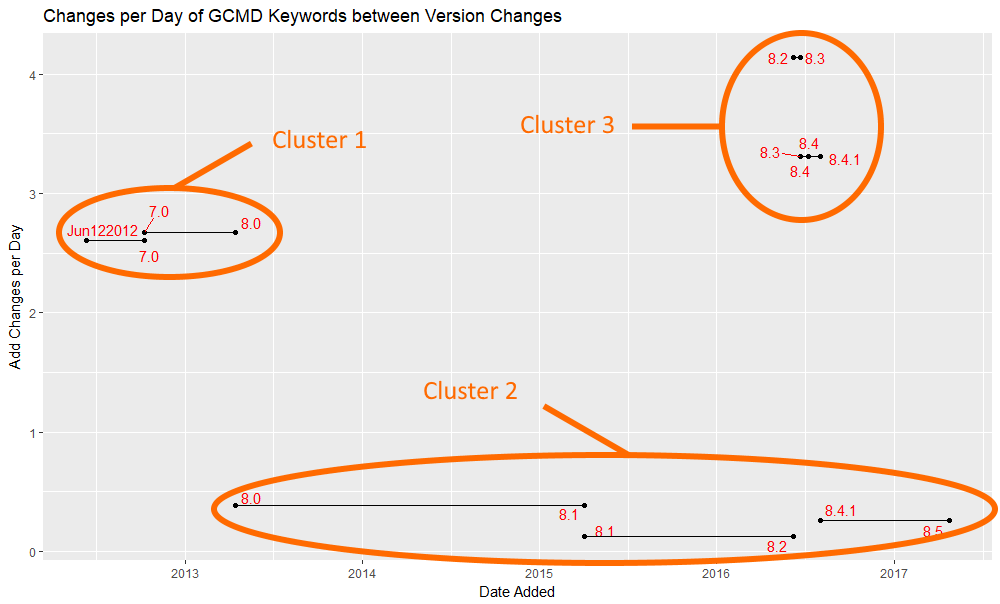
\includegraphics[scale=0.56]{figures/GCMDPlot1_Cluster.png}
	\caption[Global Change Master Directory count distributed over time with clusters marked.]{The change rate of different versions organize into three visible clusters. Cluster 2 denotes a sudden burst of version releases which is notable.}
	\label{GCMDPlot1Cluster}
\end{figure}
\begin{table}
	\caption{Global Change Master Directory versions with old start time changes.}
	\label{table:GCMD_old}
	\centering
	\begin{tabular}{|c|c|c|c|c|}
		\hline
		Version Name&	Publish Date&	2008&	2014&	2015\\ \hline
		8.2&	June 7, 2016&	0&	4&	2\\
		8.3&	June 21, 2016&	0&	7&	1\\
		8.4&	July 7, 2016&	5&	0&	1\\
		\hline
	\end{tabular}
\end{table}

\begin{table}
	\caption{Differences in VersOn and Impact Assessment metrics}
	\label{table:GCMD_metric}
	\centering
	\begin{tabular}{|r|r|r|r|}
		\hline
		Version & Add & Invalidate & Modify\\ \hline
		8.2(VO)&	53&	1&	26\\
		-8.2(IA)&	48&	0&	4\\
		\hline
		&	\textbf{5}&	\textbf{1}&	\textbf{22}\\
		\hline
		8.3(VO)&	58&	0&	13\\
		-8.3(IA)&	58&	0&	10\\
		\hline
		&	\textbf{0}&	\textbf{0}&	\textbf{3}\\
		\hline
		8.4(VO)&	53&	0&	1\\
		-8.4(IA)&	66&	0&	5\\
		\hline
		&	\textbf{-13}&	\textbf{0}&	\textbf{-4}\\
		\hline
		8.5(VO)&	68&	2&	22\\
		-8.5(IA)&	55&	0&	30\\
		\hline
		&	\textbf{13}&	\textbf{2}&	\textbf{-8}\\						
		\hline
	\end{tabular}
\end{table}

\section{Earth Observing Laboratory}

Of the 1335 data sets maintained by EOL, only 180 data sets had more than one version.  
The 1155 other data sets were filtered out since change counts could not be computed for those collections.  
The data managers indicated that when a new version is received, the entire data set is replaced.  
Since a unique file identifier like a hash sum was unavailable, all files that matched file names across versions were considered modified.  
The approach will overcount the number of modifications, but provides an upper bound on the data set volatility in the repository.  
Each count is then normalized by the number of files in the previous version to standardize comparison between data sets regardless of data set size.  
The average for each data set is taken for each change type.

\section{EOL Versioning Behavior}

The data surprisingly indicates that data sets primarily gravitate towards complete addition and invalidation.  The Additions also seem to show a tendency to add either small portions of the dataset or extremely large numbers of new files.  The rightmost bar in Figure XX counts the number of outliers in Additions.  The invalidation and modification charts also show a small normalization around 0.5, but primarily revolution around 0 or 1.

The high concentration of data sets towards 1 in additions and invalidations suggests a more complicated interaction within the data sets.  Instead of separating the counts into isolated dimensions, Figure XX groups unnormalized change counts for each version into a coordinate.  Notice the one-to-one trend between Adds and Invalidates which shows the tendency of data sets to replace every file and assign a new filename.  The files are more likely to be replaced when only a few files in a data set are being modified.

\begin{table}
	\caption{Version Content of Earth Observing Laboratory Data Sets}
	\label{table:EOL_Versions}
	\centering
	\begin{tabular}{|c|c|}
		\hline
		Number of Versions& Number of Data Sets\\ \hline
		1&	1155\\
		2&	141\\
		3&	26\\
		4&	10\\
		5&	3\\
		Total&	1335\\
		\hline
	\end{tabular}
\end{table}

\begin{table}
	\caption{Normalized Change Statistics}
	\label{table:EOL_Change}
	\centering
	\begin{tabular}{|c|c|c|c|}
		\hline
		Stat&	Add&	Invalidate&	Modify\\
		Mean&	0.714312707&	0.654819294&	0.345180706\\
		Std. Dev&	0.509878564&	0.420093557&	0.420093557\\
		Min&	0&	0&	0\\
		Q1&	0.28635075&	0.142857&	0\\
		Med&	0.9146635&	0.9642855&	0.0357145\\
		Q3&	1.00358625&	1&	0.857143\\
		Max&	54.25&	1&	1\\
		IQR&	0.7172355&	0.857143&	0.857143\\
		\hline
	\end{tabular}
\end{table}

\begin{figure}%[b]
	\centering
	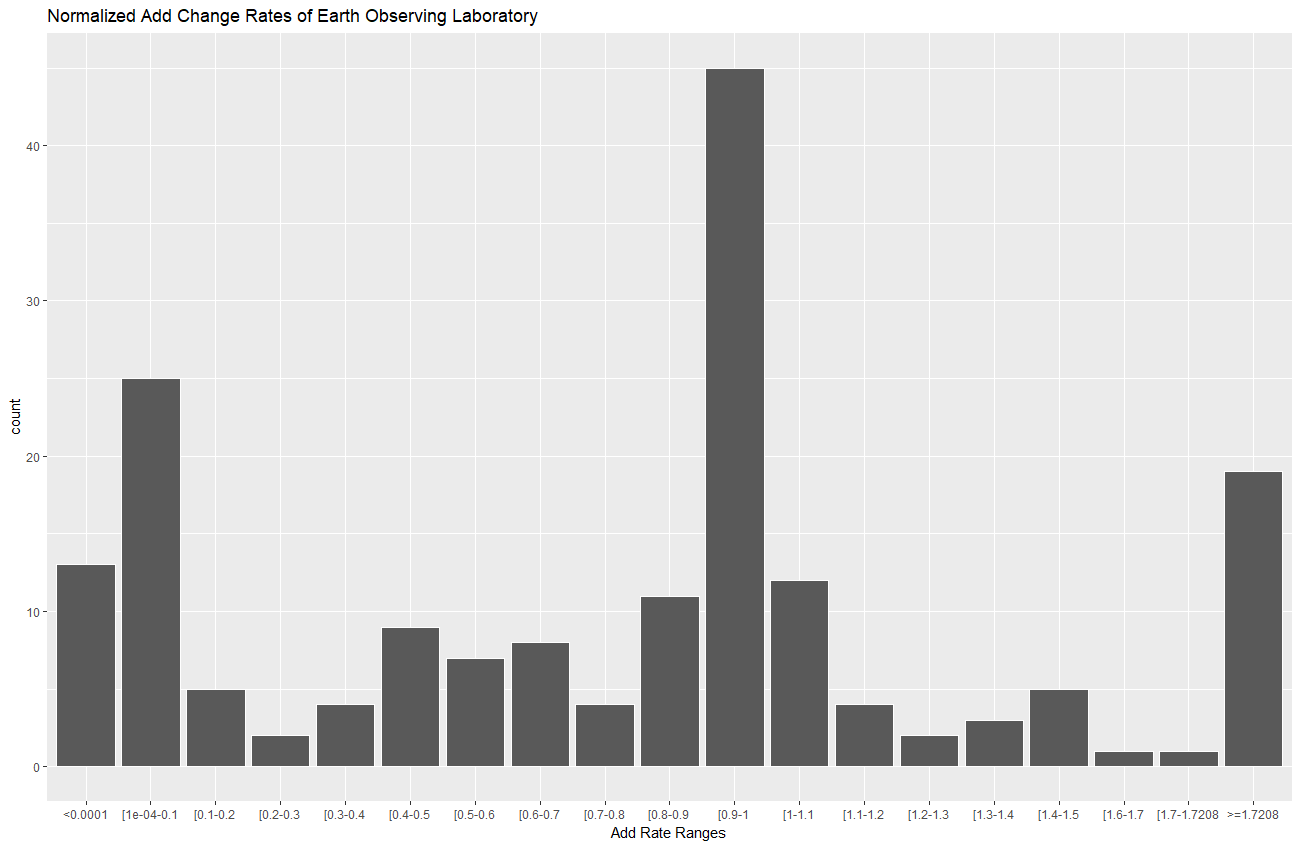
\includegraphics[scale=.43]{figures/Eol_Adds.png}
	\caption{Distribution of average normalized Add counts for each data set in Eath Observing Laboratory.}
	\label{EOL_Adds}
\end{figure}

\begin{figure}%[b]
	\centering
	\includegraphics[scale=.6]{figures/Eol_Inv.png}
	\caption{Distribution of average normalized Invalidate counts for each data set in Eath Observing Laboratory.}
	\label{EOL_Invs}
\end{figure}

\begin{figure}%[b]
	\centering
	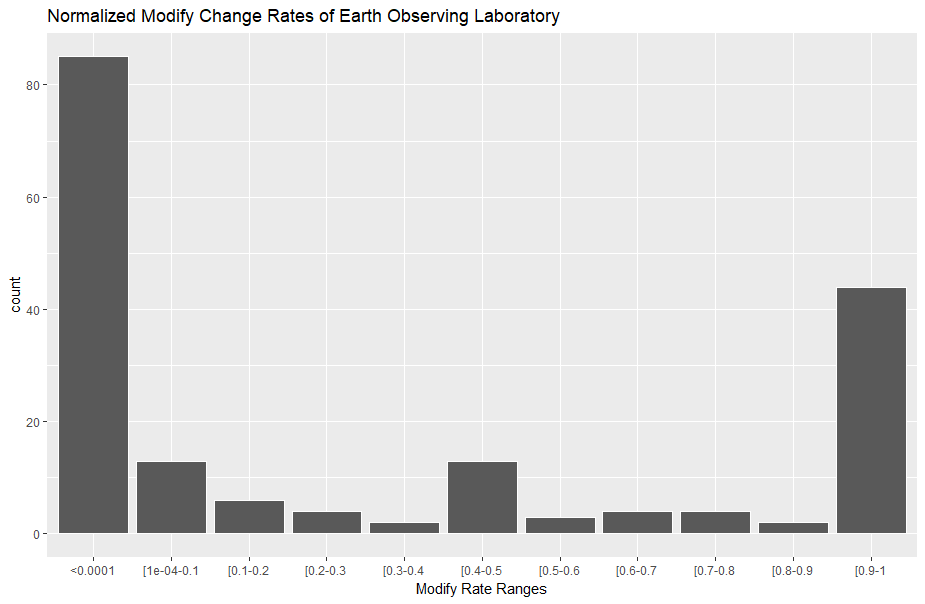
\includegraphics[scale=.6]{figures/Eol_Mod.png}
	\caption{Distribution of average normalized Modify counts of each data set in Eath Observing Laboratory.}
	\label{EOL_Mods}
\end{figure}

\begin{figure}%[b]
	\centering
	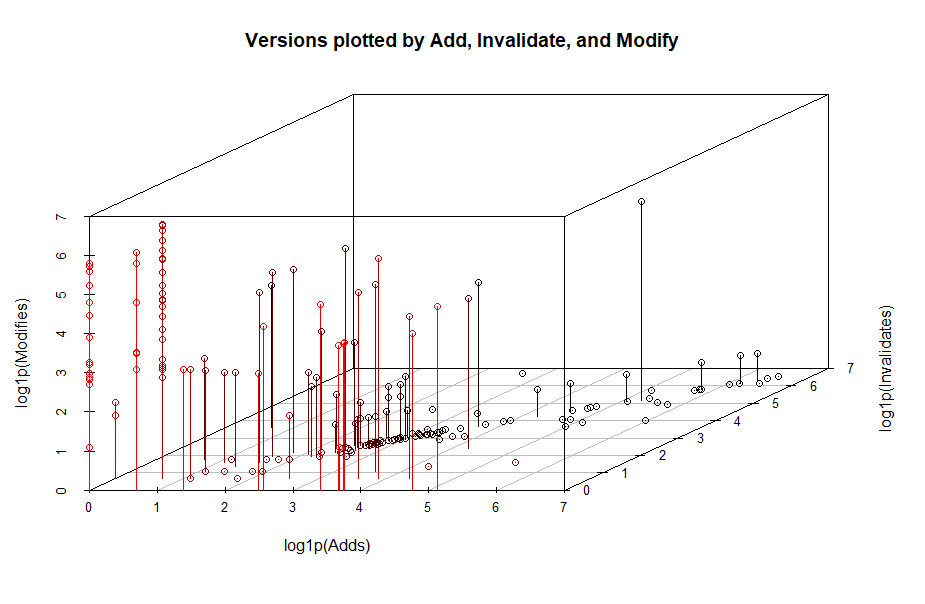
\includegraphics[scale=.6]{figures/Eol_Versions_3d.png}
	\caption{Distribution of average normalized Modify counts of each data set in Eath Observing Laboratory.}
	\label{EOL_AIM}
\end{figure}

\section{Hidden Volatility}

Each version of a data set stored in EOL is assigned three different times, “version publish time,” “version creation time,” and “version modification time.”  
Version publish time indicates the time the version was made available to the public, usually the data set was added to the database.  
Version creation time denotes the moment at which a version designation was given to the collection of files, beginning in mid-2014 when the versioning system was implemented.  
Version modification time indicates the time at which the version metadata was changed.  
Using version publish time most closely resembles the duration of version validity, and the following computations use version publish time.

Some of the data needed to be filtered out to provide valid results.  
Due to a few coding errors in time assignments, 7 versions had to be removed because the durations were negative.  
Duration is measured in days, and the rate of version publication is determined by taking the inverse of the duration.  
To acquire the AIM change rates, the changes are divided by the associated duration for each version.  
Since the rates are closely concentrated at 0, the log of the rates are taken to give the values a more log-normal distribution.  
Values where an AIM change is 0 had to be removed in order to properly apply the log function.  
The remaining number of entries can be found in Table XX.

Since the durations are not normally distributed, but concentrated close to 0, the log of the durations are taken to normalize the data.  
The log function is also applied to the AIM changes to normalize the data.  
The inverse of the log of the duration is taken to acquire the rate of version release.

The Kolomogorov-Smirnov Test was used to determine if the Adds, Invalidates, or Modifies follow a distribution separate from the version publication distribution.  
A difference indicates that the AIM changes exhibit a behavior apart from the version releases.  
As seen in Figures XX, XX, and XX, the distributions of AIM changes over duration are offset due to a larger magnitude of values per version.  
The change rates were translated by the difference in means between the version mean and the associated change mean after log normalization to make the values valid for comparison by the Kolomogorov-Smirnov test.


\begin{figure}%[b]
	\centering
	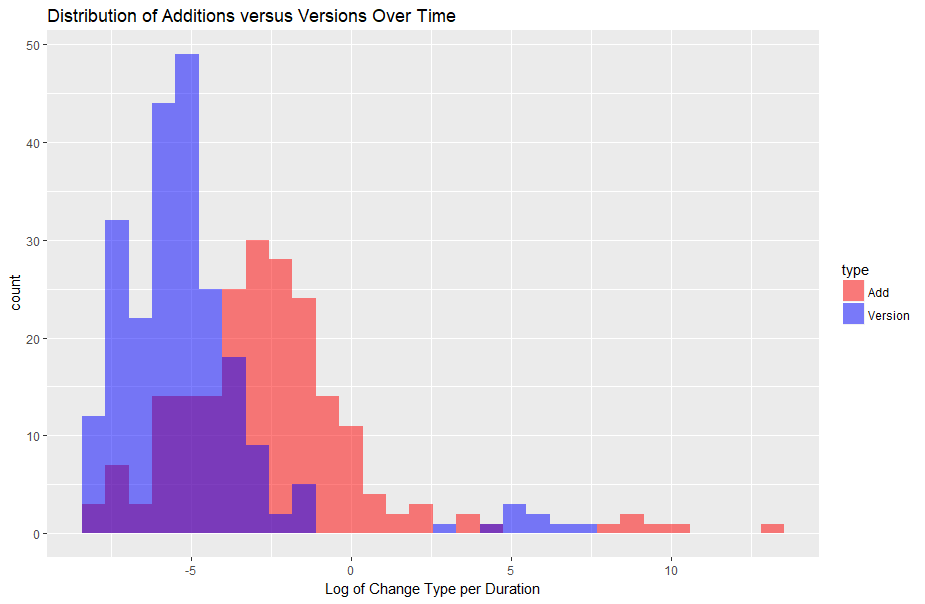
\includegraphics[scale=.6]{figures/Eol_Add_Ver_Rate.png}
	\caption{Distribution of average normalized Modify counts of each data set in Eath Observing Laboratory.}
	\label{EOL_Add_Ver}
\end{figure}

\begin{figure}%[b]
	\centering
	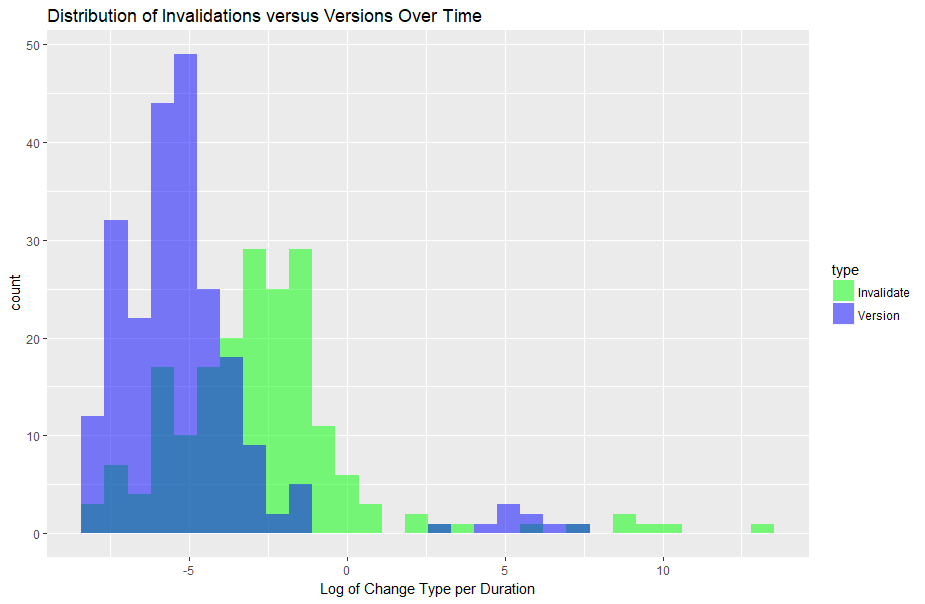
\includegraphics[scale=.6]{figures/Eol_Inv_Ver_Rate.png}
	\caption{Distribution of average normalized Modify counts of each data set in Eath Observing Laboratory.}
	\label{EOL_Inv_Ver}
\end{figure}

\begin{figure}%[b]
	\centering
	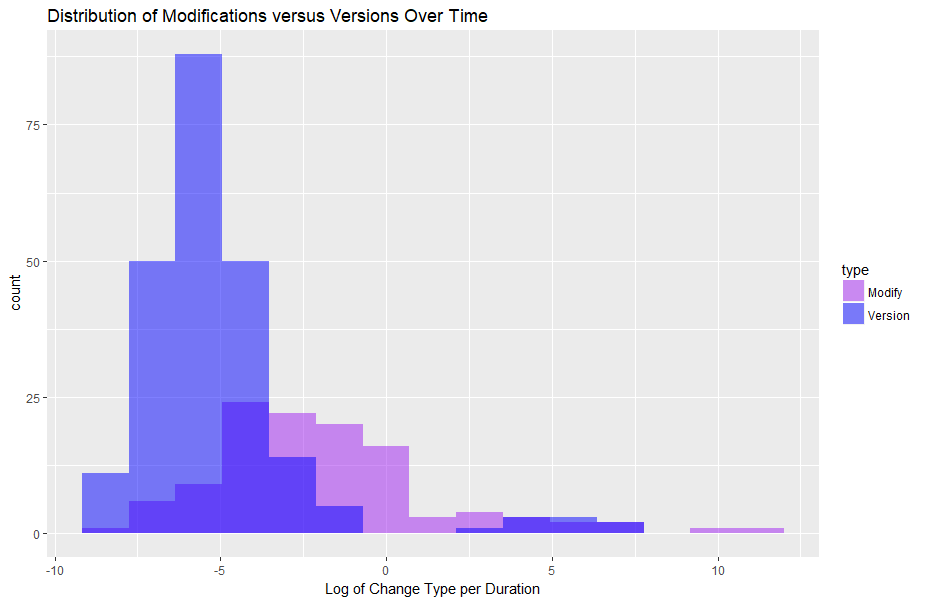
\includegraphics[scale=.6]{figures/Eol_Mod_Ver_Rate.png}
	\caption{Distribution of average normalized Modify counts of each data set in Eath Observing Laboratory.}
	\label{EOL_Mod_Ver}
\end{figure}

\begin{table}
	\caption{Summary of Kolmogorov-Smirnov Test results for Earth Observing Laboratory.}
	\label{table:Eol_KS}
	\centering
	\begin{tabular}{|c|c|c|c|c|}
		\hline
		&	Add&	Invalidate&	Modify&	Versions\\ \hline
		Length&	205&	192&	114&	227\\
		D-Value&	0.12919&	0.14464&	0.19727&	NA\\
		p-Value&	0.05487&	0.02575&	0.005443&	NA\\
		\hline
	\end{tabular}
\end{table}